\documentclass[10pt]{beamer}\usepackage{graphicx, color}
%% maxwidth is the original width if it is less than linewidth
%% otherwise use linewidth (to make sure the graphics do not exceed the margin)
\makeatletter
\def\maxwidth{ %
  \ifdim\Gin@nat@width>\linewidth
    \linewidth
  \else
    \Gin@nat@width
  \fi
}
\makeatother

\definecolor{fgcolor}{rgb}{0.2, 0.2, 0.2}
\newcommand{\hlfunctioncall}[1]{\textcolor[rgb]{0,0,0.545098039215686}{\textbf{#1}}}%
\newcommand{\hlstring}[1]{\textcolor[rgb]{0.282352941176471,0.23921568627451,0.545098039215686}{#1}}%
\newcommand{\hlnumber}[1]{\textcolor[rgb]{0,0,0}{#1}}%
\newcommand{\hlkeyword}[1]{\textcolor[rgb]{0,0,0}{\textbf{#1}}}%
\newcommand{\hlargument}[1]{\textcolor[rgb]{0.690196078431373,0.250980392156863,0.0196078431372549}{#1}}%
\newcommand{\hlcomment}[1]{\textcolor[rgb]{0.2,0.2,0.2}{#1}}%
\newcommand{\hlroxygencomment}[1]{\textcolor[rgb]{0.2,0.2,0.2}{#1}}%
\newcommand{\hlformalargs}[1]{\textcolor[rgb]{0.690196078431373,0.250980392156863,0.0196078431372549}{#1}}%
\newcommand{\hleqformalargs}[1]{\textcolor[rgb]{0.690196078431373,0.250980392156863,0.0196078431372549}{#1}}%
\newcommand{\hlassignement}[1]{\textcolor[rgb]{0,0,0}{\textbf{#1}}}%
\newcommand{\hlpackage}[1]{\textcolor[rgb]{0.588235294117647,0.709803921568627,0.145098039215686}{#1}}%
\newcommand{\hlslot}[1]{\textit{#1}}%
\newcommand{\hlsymbol}[1]{\textcolor[rgb]{0,0,0}{#1}}%
\newcommand{\hlprompt}[1]{\textcolor[rgb]{0.2,0.2,0.2}{#1}}%

\usepackage{framed}
\makeatletter
\newenvironment{kframe}{%
 \def\at@end@of@kframe{}%
 \ifinner\ifhmode%
  \def\at@end@of@kframe{\end{minipage}}%
  \begin{minipage}{\columnwidth}%
 \fi\fi%
 \def\FrameCommand##1{\hskip\@totalleftmargin \hskip-\fboxsep
 \colorbox{shadecolor}{##1}\hskip-\fboxsep
     % There is no \\@totalrightmargin, so:
     \hskip-\linewidth \hskip-\@totalleftmargin \hskip\columnwidth}%
 \MakeFramed {\advance\hsize-\width
   \@totalleftmargin\z@ \linewidth\hsize
   \@setminipage}}%
 {\par\unskip\endMakeFramed%
 \at@end@of@kframe}
\makeatother

\definecolor{shadecolor}{rgb}{.97, .97, .97}
\definecolor{messagecolor}{rgb}{0, 0, 0}
\definecolor{warningcolor}{rgb}{1, 0, 1}
\definecolor{errorcolor}{rgb}{1, 0, 0}
\newenvironment{knitrout}{}{} % an empty environment to be redefined in TeX

\usepackage{alltt}

\usetheme[compress]{PaloAlto}
\usecolortheme{sidebartab}
%\logo{
\includegraphics[width=1cm]{../Rlogo-5.png}}

\usepackage[brazilian]{babel}
\usepackage[T1]{fontenc}
\usepackage[utf8]{inputenc}
\usepackage{graphicx}
\usepackage{hyperref}
\usepackage[scaled]{beramono} % truetype: Bistream Vera Sans Mono
%\usepackage{inconsolata}

\setbeamertemplate{footline}[frame number] % mostra o numero dos slides
\setbeamertemplate{navigation symbols}{} % retira a barra de navegacao

\usepackage{xspace}
\providecommand{\eg}{\textit{e.g.}\xspace}
\providecommand{\ie}{\textit{i.e.}\xspace}
%\providecommand{\R}{\texttt{R}\xspace}

\title[Módulo II\\ Descritiva]{Introdução ao uso do software R}
\author[]{Fernando de Pol Mayer\inst{1} \and %\url{fernandomayer@gmail.com} \and
Rodrigo Sant'Ana\inst{2}} %\\ \url{oc.rodrigosantana@gmail.com}}
\date{26 e 27 de Novembro, 2012}
\institute{
  \inst{1}%
  Universidade Federal de Santa Catarina (UFSC) \\
  Departamento de Ecologia e Zoologia (ECZ/CCB) \\
  \url{fernando.mayer@gmail.com}
  \and
  \inst{2}%
  Instituto Albatroz \\
  \url{oc.rodrigosantana@gmail.com}
}
\logo{
\includegraphics[width=1cm]{../Rlogo-5}}

\AtBeginSection[]
{
  \begin{frame}
    \frametitle{Sumário}
    \tableofcontents[currentsection]
  \end{frame}
}

\AtBeginSubsection[]
{
  \begin{frame}
    \frametitle{Sumário}
    \tableofcontents[currentsection,currentsubsection]
  \end{frame}
}

\begin{document}




\begin{frame}
\maketitle
%\titlepage
\end{frame}

\begin{frame}{Sumário}
\tableofcontents
\end{frame}

\section{Importação de dados}

\begin{frame}[fragile=singleslide]{Antes de importar para o R}
\begin{itemize}
\item Se houverem valores perdidos, preencha com \texttt{NA}s
\item A matriz de dados deve formar um bloco só. Se houverem colunas de
  diferentes comprimentos, preencha com \texttt{NA}s
\item Salve o arquivo como ``valores separados por vírgula''
  (\texttt{.csv}), mas atenção:
    \begin{itemize}
    \item Se o separador de decimal for ``\texttt{,}'', o separador de
      campos será ``\texttt{;}'' automaticamente (o que é mais comum nos
      sistemas em português).
    \end{itemize}
\end{itemize}
\end{frame}

%% \begin{frame}[fragile=singleslide]{O editor de scripts}
%% \begin{itemize}
%% \item Para criar rotinas computacionais é necessário utilizar um editor
%%   de scripts.
%% \item Clique em \texttt{Arquivo > Novo script}. Salve com a extensão
%%   \texttt{.R}.
%% \item Para enviar comandos diretamente para o console, selecione-os e
%%   aperte \texttt{Ctrl + R}.
%% \item Para adicionar comentários ao script, utiliza-se o símbolo
%%   \texttt{\#} antes do texto e/ou comandos. O que estiver depois do
%%   símbolo não será interpretado pelo R. Portanto:
%% \begin{verbatim}
%% 2 + 2     # esta linha será executada
%% # 2 + 2     esta linha não será executada
%% \end{verbatim}
%% \end{itemize}
%% \end{frame}

\begin{frame}[fragile=singleslide]{A função \texttt{read.table()}}
O método mais comum de importação de dados para o R, é utilizando a
função \texttt{read.table()}. Para importar um arquivo \texttt{.csv}
faça:
\begin{knitrout}\small
\definecolor{shadecolor}{rgb}{0.933, 0.914, 0.914}\color{fgcolor}\begin{kframe}
\begin{alltt}
> dados <- \hlfunctioncall{read.table}(\hlstring{"crabs.csv"}, header = T, sep = \hlstring{";"},
                      dec = \hlstring{","})
\end{alltt}
\end{kframe}
\end{knitrout}

Argumentos:
\begin{itemize}
\item \verb|"crabs.csv"|: nome do arquivo
\item \texttt{header = T}: significa que a primeira linha do arquivo deve
  ser inrpretada como os nomes das colunas
\item \texttt{sep = ";"}: o separador de colunas (também pode ser
  \verb|"\t"| para tabulação e \verb|""| para espaços)
\item \texttt{dec = ","}: o separador de decimais
\end{itemize}
\end{frame}

\begin{frame}[fragile=singleslide]{Estrutura dos dados importados}
A função \texttt{str()} serve para demonstrar a estrutura de um objeto,
como o nome das colunas e suas classes:
\begin{knitrout}\small
\definecolor{shadecolor}{rgb}{0.933, 0.914, 0.914}\color{fgcolor}\begin{kframe}
\begin{alltt}
> \hlfunctioncall{str}(dados)
\end{alltt}
\begin{verbatim}
'data.frame':	156 obs. of  7 variables:
 $ especie: Factor w/ 2 levels "azul","laranja": 1 1 1 1 1 1 1 1 1 1 ...
 $ sexo   : Factor w/ 2 levels "F","M": 2 2 2 2 2 2 2 2 2 2 ...
 $ FL     : num  8.1 8.8 9.2 9.6 10.8 11.6 11.8 12.3 12.6 12.8 ...
 $ RW     : num  6.7 7.7 7.8 7.9 9 9.1 10.5 11 10 10.9 ...
 $ CL     : num  16.1 18.1 19 20.1 23 24.5 25.2 26.8 27.7 27.4 ...
 $ CW     : num  19 20.8 22.4 23.1 26.5 28.4 29.3 31.5 31.7 31.5 ...
 $ BD     : num  7 7.4 7.7 8.2 9.8 10.4 10.3 11.4 11.4 11 ...
\end{verbatim}
\end{kframe}
\end{knitrout}

\end{frame}

\begin{frame}[fragile=singleslide]{Estrutura dos dados importados}
Para visualizar as 10 primeiras linhas do data frame:
\begin{knitrout}\small
\definecolor{shadecolor}{rgb}{0.933, 0.914, 0.914}\color{fgcolor}\begin{kframe}
\begin{alltt}
> \hlfunctioncall{head}(dados, 10) \hlcomment{# ou: dados[1:10,]}
\end{alltt}
\begin{verbatim}
   especie sexo   FL   RW   CL   CW   BD
1     azul    M  8.1  6.7 16.1 19.0  7.0
2     azul    M  8.8  7.7 18.1 20.8  7.4
3     azul    M  9.2  7.8 19.0 22.4  7.7
4     azul    M  9.6  7.9 20.1 23.1  8.2
5     azul    M 10.8  9.0 23.0 26.5  9.8
6     azul    M 11.6  9.1 24.5 28.4 10.4
7     azul    M 11.8 10.5 25.2 29.3 10.3
8     azul    M 12.3 11.0 26.8 31.5 11.4
9     azul    M 12.6 10.0 27.7 31.7 11.4
10    azul    M 12.8 10.9 27.4 31.5 11.0
\end{verbatim}
\end{kframe}
\end{knitrout}

\end{frame}

% \begin{frame}[fragile=singleslide]{Estrutura dos dados importados}
% Alternativamente, o editor de dados pode ser utilizado para
% visualização:
% \begin{verbatim}
% > edit(dados)
% \end{verbatim}
% Note que qualquer alteração aqui não terá efeito ao menos que este
% comando seja associado a um objeto:
% \begin{verbatim}
% > dados <- edit(dados)
% \end{verbatim}
% O comando \texttt{fix()} tem o mesmo efeito que o anterior
% (\textit{i.e.} armazena as alterações feitas no objeto \texttt{dados}):
% \begin{verbatim}
% > fix(dados)
% \end{verbatim}
% \end{frame}

\section{Estatística descrtiva}

\begin{frame}[fragile=singleslide]{Medidas de centro}
Média (utilizando a coluna \texttt{CL}):
\begin{knitrout}\small
\definecolor{shadecolor}{rgb}{0.933, 0.914, 0.914}\color{fgcolor}\begin{kframe}
\begin{alltt}
> \hlfunctioncall{mean}(dados$CL) \hlcomment{# ou \hlfunctioncall{sum}(dados$CL)/\hlfunctioncall{length}(dados$CL)}
\end{alltt}
\begin{verbatim}
[1] 32.004
\end{verbatim}
\end{kframe}
\end{knitrout}

Média (utilizando a coluna \texttt{BD}):
\begin{knitrout}\small
\definecolor{shadecolor}{rgb}{0.933, 0.914, 0.914}\color{fgcolor}\begin{kframe}
\begin{alltt}
> \hlfunctioncall{mean}(dados$BD)
\end{alltt}
\begin{verbatim}
[1] NA
\end{verbatim}
\end{kframe}
\end{knitrout}

Observe que a presença de \texttt{NA}s interfere no resultado. O
argumento \texttt{na.rm} pode ser utilizado para que o cálculo seja
feito sem os \texttt{NA}s:
\begin{knitrout}\small
\definecolor{shadecolor}{rgb}{0.933, 0.914, 0.914}\color{fgcolor}\begin{kframe}
\begin{alltt}
> \hlfunctioncall{mean}(dados$BD, na.rm=T)
\end{alltt}
\begin{verbatim}
[1] 14.019
\end{verbatim}
\end{kframe}
\end{knitrout}

O argumento \texttt{na.rm} é utilizado também em outras funções como
\texttt{median()}, \texttt{sum()} e \texttt{var()}
\end{frame}

% \begin{frame}[fragile=singleslide]{Medidas de centro}
% Mediana (coluna \texttt{CL}):
% \begin{verbatim}
% > median(dados$lage, na.rm=T)
% [1] 400
% \end{verbatim}
% Ponto médio:
% \begin{verbatim}
% > (max(dados$lage, na.rm=T) +
% +     min(dados$lage, na.rm=T))/2
% [1] 103550
% \end{verbatim}
% \end{frame}

\begin{frame}[fragile=singleslide]{Medidas de variação}
Desvio padrão (coluna \texttt{CL}):
\begin{knitrout}\small
\definecolor{shadecolor}{rgb}{0.933, 0.914, 0.914}\color{fgcolor}\begin{kframe}
\begin{alltt}
> \hlfunctioncall{sd}(dados$CL)
\end{alltt}
\begin{verbatim}
[1] 7.2278
\end{verbatim}
\end{kframe}
\end{knitrout}

Variância:
\begin{knitrout}\small
\definecolor{shadecolor}{rgb}{0.933, 0.914, 0.914}\color{fgcolor}\begin{kframe}
\begin{alltt}
> \hlfunctioncall{var}(dados$CL) \hlcomment{# \hlfunctioncall{sd}(dados$CL)^2}
\end{alltt}
\begin{verbatim}
[1] 52.242
\end{verbatim}
\end{kframe}
\end{knitrout}

Coeficiente de variação:
\begin{knitrout}\small
\definecolor{shadecolor}{rgb}{0.933, 0.914, 0.914}\color{fgcolor}\begin{kframe}
\begin{alltt}
> \hlfunctioncall{sd}(dados$CL)/\hlfunctioncall{mean}(dados$CL)
\end{alltt}
\begin{verbatim}
[1] 0.22584
\end{verbatim}
\end{kframe}
\end{knitrout}

\end{frame}

\begin{frame}[fragile=singleslide]{Medidas de posição relativa}
Quartis:
\begin{knitrout}\small
\definecolor{shadecolor}{rgb}{0.933, 0.914, 0.914}\color{fgcolor}\begin{kframe}
\begin{alltt}
> \hlfunctioncall{quantile}(dados$CL)
\end{alltt}
\begin{verbatim}
    0%    25%    50%    75%   100% 
14.700 27.075 32.300 37.050 47.600 
\end{verbatim}
\end{kframe}
\end{knitrout}

Decis:
\begin{knitrout}\small
\definecolor{shadecolor}{rgb}{0.933, 0.914, 0.914}\color{fgcolor}\begin{kframe}
\begin{alltt}
> \hlfunctioncall{quantile}(dados$CL, probs = \hlfunctioncall{seq}(0, 1, 0.1))
\end{alltt}
\begin{verbatim}
   0%   10%   20%   30%   40%   50%   60%   70%   80%   90% 
14.70 22.10 25.40 28.15 30.10 32.30 34.20 36.10 38.10 41.40 
 100% 
47.60 
\end{verbatim}
\end{kframe}
\end{knitrout}

\end{frame}

\begin{frame}[fragile=singleslide]{Sumários}
A função \texttt{summary()} resume os dados de forma lógica:
\begin{knitrout}\small
\definecolor{shadecolor}{rgb}{0.933, 0.914, 0.914}\color{fgcolor}\begin{kframe}
\begin{alltt}
> \hlfunctioncall{summary}(dados$CL)
\end{alltt}
\begin{verbatim}
   Min. 1st Qu.  Median    Mean 3rd Qu.    Max. 
   14.7    27.1    32.3    32.0    37.0    47.6 
\end{verbatim}
\end{kframe}
\end{knitrout}

\texttt{1st Qu.} e \texttt{3rd Qu.} se referem ao $1^{o}$ e $3^{o}$
quartis. Se houverem \texttt{NA}s, eles também serão contados:
\begin{knitrout}\small
\definecolor{shadecolor}{rgb}{0.933, 0.914, 0.914}\color{fgcolor}\begin{kframe}
\begin{alltt}
> \hlfunctioncall{summary}(dados$BD)
\end{alltt}
\begin{verbatim}
   Min. 1st Qu.  Median    Mean 3rd Qu.    Max.    NA's 
    6.1    11.5    13.8    14.0    16.6    21.6       2 
\end{verbatim}
\end{kframe}
\end{knitrout}

\end{frame}

\begin{frame}[fragile=singleslide]{Sumários}
A função \texttt{summary()} pode ser utilizada para resumir todo o data frame:
\begin{knitrout}\small
\definecolor{shadecolor}{rgb}{0.933, 0.914, 0.914}\color{fgcolor}\begin{kframe}
\begin{alltt}
> \hlfunctioncall{summary}(dados)
\end{alltt}
\begin{verbatim}
    especie   sexo         FL             RW      
 azul   :77   F:87   Min.   : 7.2   Min.   : 6.5  
 laranja:79   M:69   1st Qu.:12.9   1st Qu.:11.0  
                     Median :15.6   Median :12.8  
                     Mean   :15.6   Mean   :12.8  
                     3rd Qu.:18.2   3rd Qu.:14.5  
                     Max.   :23.1   Max.   :20.2  
                     NA's   :2                    
       CL             CW             BD      
 Min.   :14.7   Min.   :17.1   Min.   : 6.1  
 1st Qu.:27.1   1st Qu.:31.4   1st Qu.:11.5  
 Median :32.3   Median :36.9   Median :13.8  
 Mean   :32.0   Mean   :36.3   Mean   :14.0  
 3rd Qu.:37.0   3rd Qu.:41.9   3rd Qu.:16.6  
 Max.   :47.6   Max.   :54.6   Max.   :21.6  
                               NA's   :2     
\end{verbatim}
\end{kframe}
\end{knitrout}

\end{frame}

\begin{frame}[fragile=singleslide]{Tabelas de contingência}
A função \texttt{table()} é usada para formar tabelas de contingência:
\begin{knitrout}\small
\definecolor{shadecolor}{rgb}{0.933, 0.914, 0.914}\color{fgcolor}\begin{kframe}
\begin{alltt}
> \hlfunctioncall{table}(dados$especie)
\end{alltt}
\begin{verbatim}

   azul laranja 
     77      79 
\end{verbatim}
\end{kframe}
\end{knitrout}

Pode também ser utilizada para a contagem de combinações de fatores:
\begin{knitrout}\small
\definecolor{shadecolor}{rgb}{0.933, 0.914, 0.914}\color{fgcolor}\begin{kframe}
\begin{alltt}
> \hlfunctioncall{table}(dados$especie, dados$sexo)
\end{alltt}
\begin{verbatim}
         
           F  M
  azul    43 34
  laranja 44 35
\end{verbatim}
\end{kframe}
\end{knitrout}

\end{frame}

\begin{frame}[fragile=singleslide]{As funções \texttt{*apply()}}
A função \texttt{lapply()} retorna uma lista com os resultados de uma
função aplicada a elemento(s) de um data frame:
\begin{knitrout}\small
\definecolor{shadecolor}{rgb}{0.933, 0.914, 0.914}\color{fgcolor}\begin{kframe}
\begin{alltt}
> \hlfunctioncall{lapply}(dados[, 3:7], mean) \hlcomment{# na.rm = T para lidar com NAs}
\end{alltt}
\begin{verbatim}
$FL
[1] NA

$RW
[1] 12.815

$CL
[1] 32.004

$CW
[1] 36.31

$BD
[1] NA

\end{verbatim}
\end{kframe}
\end{knitrout}

\texttt{sapply()} simplifica os resultados em um vetor:
\begin{knitrout}\small
\definecolor{shadecolor}{rgb}{0.933, 0.914, 0.914}\color{fgcolor}\begin{kframe}
\begin{alltt}
> \hlfunctioncall{sapply}(dados[, 3:7], mean, na.rm = T)
\end{alltt}
\begin{verbatim}
    FL     RW     CL     CW     BD 
15.577 12.815 32.004 36.310 14.019 
\end{verbatim}
\end{kframe}
\end{knitrout}

\end{frame}

\begin{frame}[fragile=singleslide]{As funções \texttt{*apply()}}
\texttt{sapply()} simplifica os resultados em um vetor:
\begin{knitrout}\small
\definecolor{shadecolor}{rgb}{0.933, 0.914, 0.914}\color{fgcolor}\begin{kframe}
\begin{alltt}
> \hlfunctioncall{sapply}(dados[, 3:7], mean, na.rm = T)
\end{alltt}
\begin{verbatim}
    FL     RW     CL     CW     BD 
15.577 12.815 32.004 36.310 14.019 
\end{verbatim}
\end{kframe}
\end{knitrout}

\texttt{apply()} aplica a função especificada por linha (\texttt{1}) ou
coluna (\texttt{2}):
\begin{knitrout}\small
\definecolor{shadecolor}{rgb}{0.933, 0.914, 0.914}\color{fgcolor}\begin{kframe}
\begin{alltt}
> \hlfunctioncall{apply}(dados[, 3:7], 2, mean, na.rm=T)
\end{alltt}
\begin{verbatim}
    FL     RW     CL     CW     BD 
15.577 12.815 32.004 36.310 14.019 
\end{verbatim}
\end{kframe}
\end{knitrout}

\end{frame}

\begin{frame}[fragile=singleslide]{As funções \texttt{*apply()}}
A função \texttt{tapply()} aplica a função (\texttt{mean}) a um vetor
(\texttt{dados\$CL}) para cada combinação dos níveis dos fatores
(\texttt{list()}):
\begin{knitrout}\small
\definecolor{shadecolor}{rgb}{0.933, 0.914, 0.914}\color{fgcolor}\begin{kframe}
\begin{alltt}
> \hlfunctioncall{tapply}(dados$CL, \hlfunctioncall{list}(dados$especie, dados$sexo), mean)
\end{alltt}
\begin{verbatim}
             F      M
azul    28.044 32.176
laranja 34.570 33.474
\end{verbatim}
\end{kframe}
\end{knitrout}

\end{frame}

\begin{frame}[fragile=singleslide]{A função \texttt{aggregate()} (``tabela dinâmica'')}
A função \texttt{aggregate()} agrega valores utilizando uma função, de
acordo com uma lista de fatores especificados:
\begin{knitrout}\small
\definecolor{shadecolor}{rgb}{0.933, 0.914, 0.914}\color{fgcolor}\begin{kframe}
\begin{alltt}
> \hlfunctioncall{aggregate}(\hlfunctioncall{cbind}(FL, RW, CL, CW, BD) ~ especie + sexo,
            data = dados, median, na.rm=T)
\end{alltt}
\begin{verbatim}
  especie sexo   FL   RW    CL    CW   BD
1    azul    F 13.3 12.2 28.15 32.65 11.8
2 laranja    F 18.0 14.6 34.70 39.40 15.7
3    azul    M 15.3 12.0 32.75 37.35 13.6
4 laranja    M 16.3 12.0 32.30 35.30 14.7
\end{verbatim}
\end{kframe}
\end{knitrout}

\end{frame}

\section{Análise gráfica}

\begin{frame}[fragile=singleslide]{Gráficos}
Os comandos para gráficos se dividem em três grupos:
\begin{itemize}
\item \textbf{Alto-nível}: são as funções que criam novos gráficos, com
  eixos, títulos, etc. Exemplo: \texttt{plot()}, \texttt{hist()},
  \texttt{barplot()}
\item \textbf{Baixo-nível}: funções que adicionam mais informações
  (pontos, linhas, texto, etc.) a um gráfico já existente Exemplo:
  \texttt{lines()}, \texttt{points()}, \texttt{legend()}
\item \textbf{Interativo}: funções que permitem adicionar ou extrair
  informações a um gráfico já existente, de modo interativo. Exemplo:
  \texttt{locator()}
\end{itemize}
Ainda existem uma série de parâmetros gráficos que podem ser manipulados
e customizados.
\end{frame}

\begin{frame}[fragile=singleslide]{Gráficos}{Terminologia}
\begin{figure}[htp]
\centering
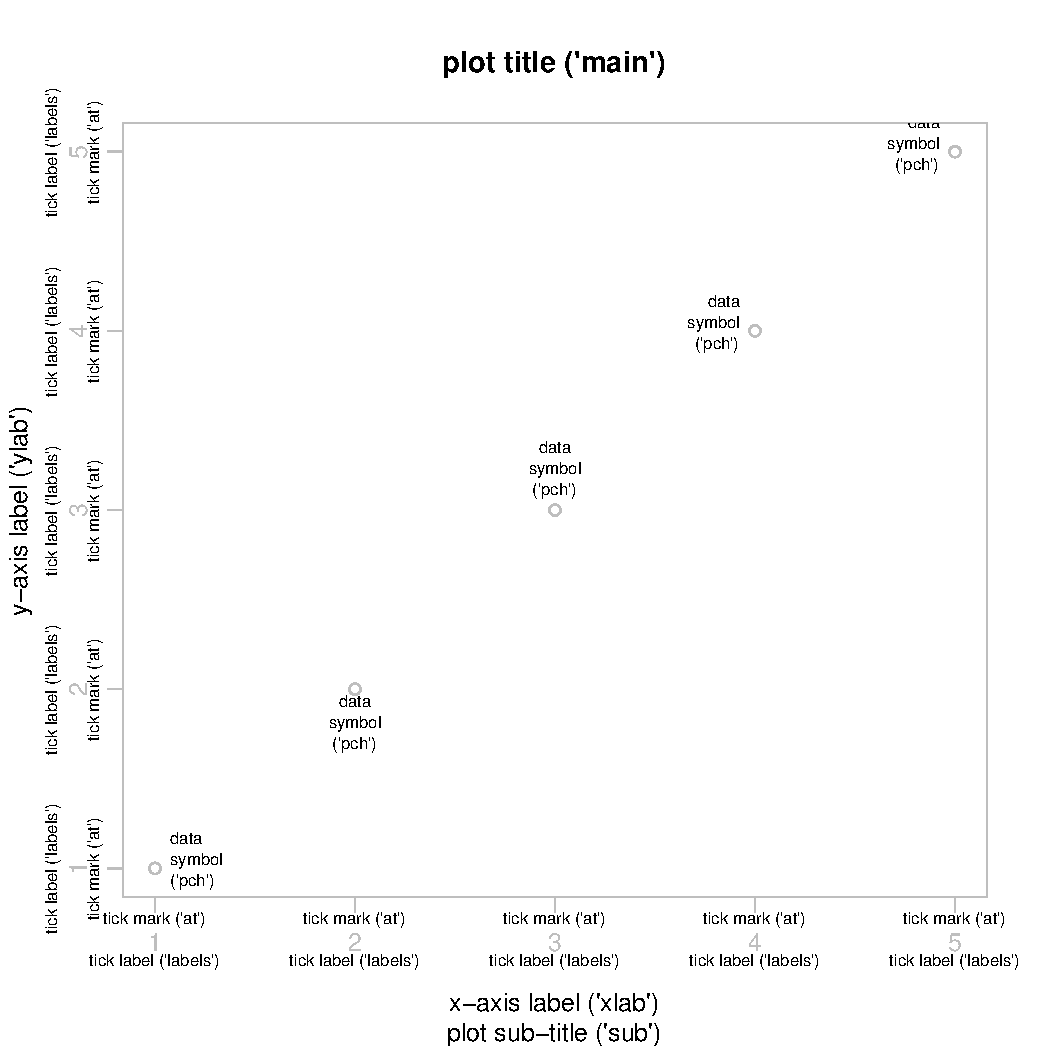
\includegraphics[height=0.95\textheight]{fig8m}
\end{figure}
\end{frame}

\begin{frame}[fragile=singleslide]{Gráficos}{Regiões do gráfico}
\begin{figure}[htp]
\centering
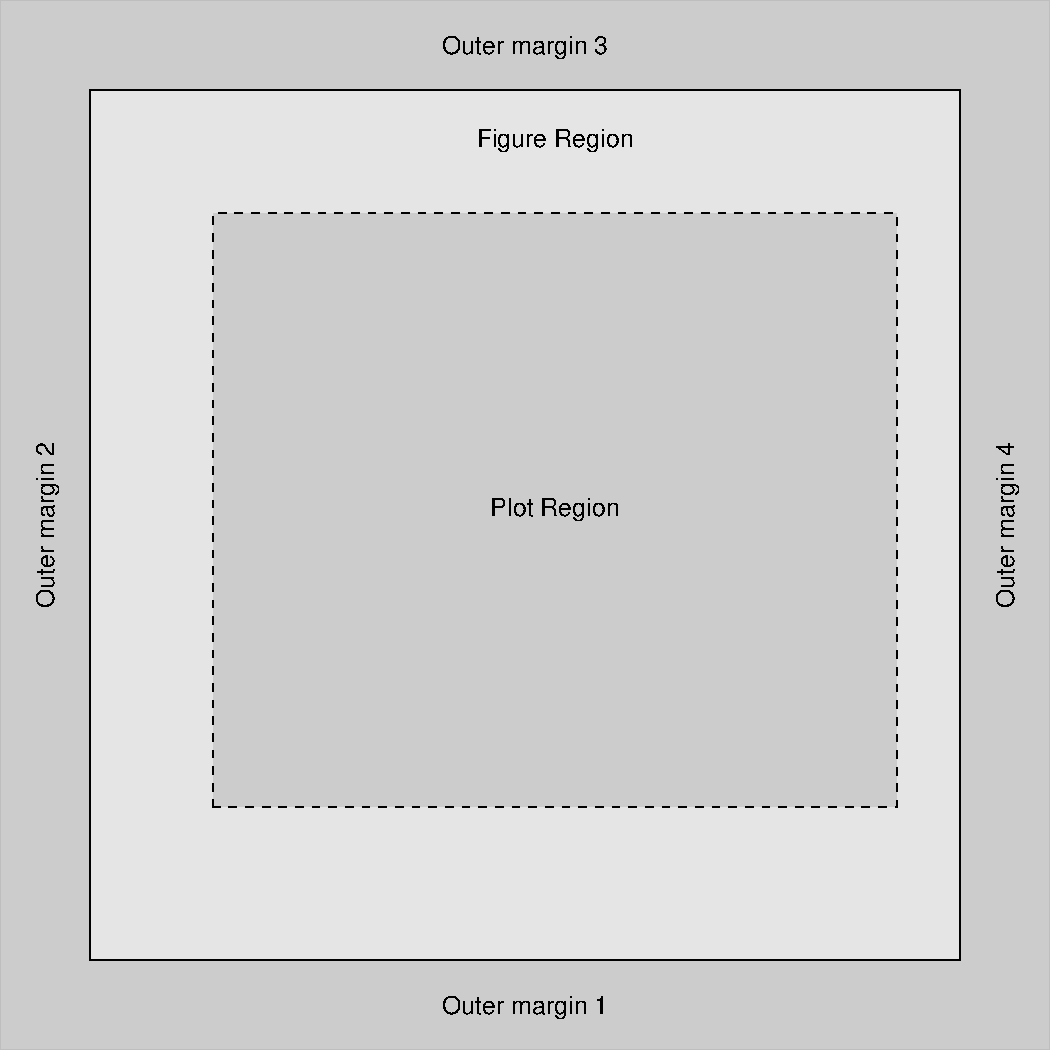
\includegraphics[height=0.95\textheight]{fig1m}
\end{figure}
\end{frame}

\begin{frame}[fragile=singleslide]{Gráficos}{Regiões de múltiplos
    gráficos}
\begin{figure}[htp]
\centering
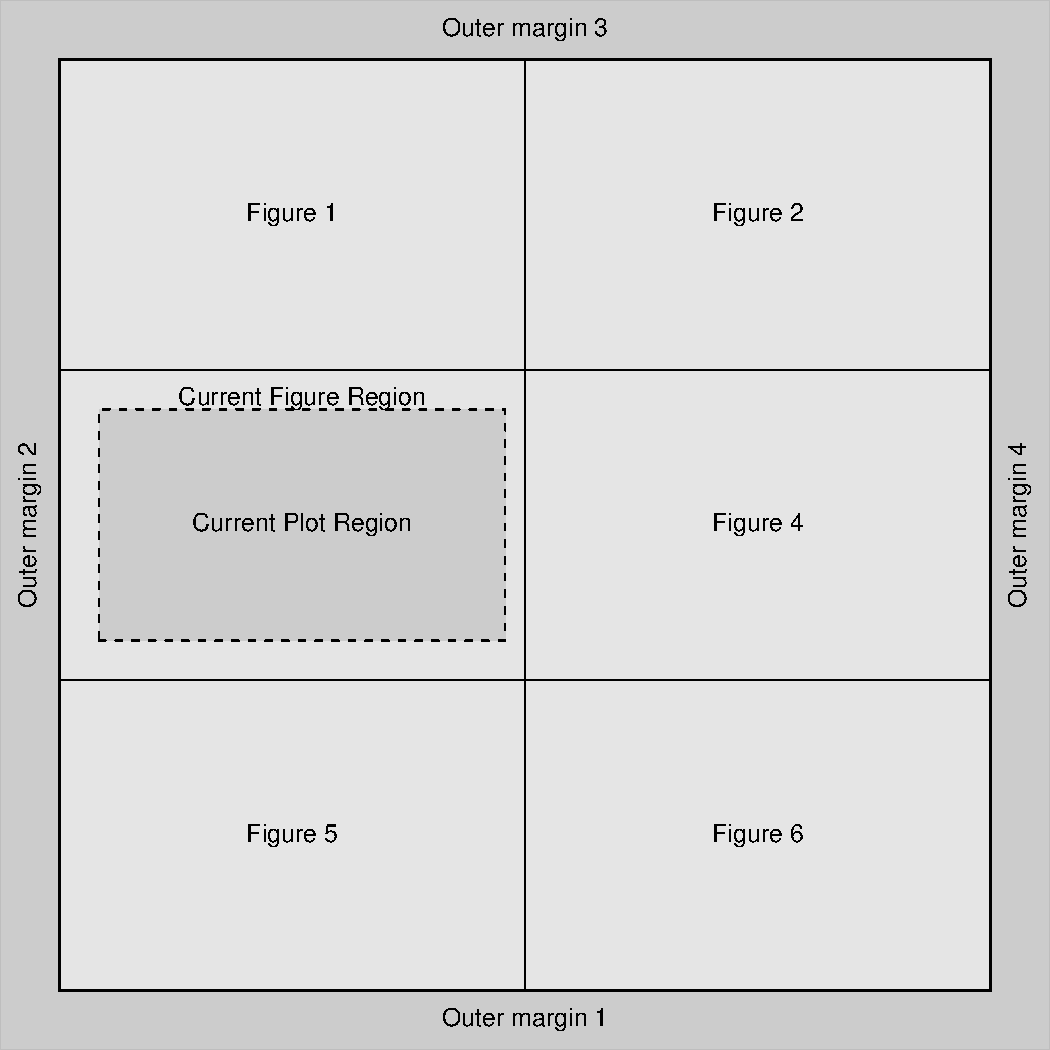
\includegraphics[height=0.95\textheight]{fig2m}
\end{figure}
\end{frame}

\begin{frame}[fragile=singleslide]{Gráficos}{Sistema de coordenadas}
\begin{figure}[htp]
\centering
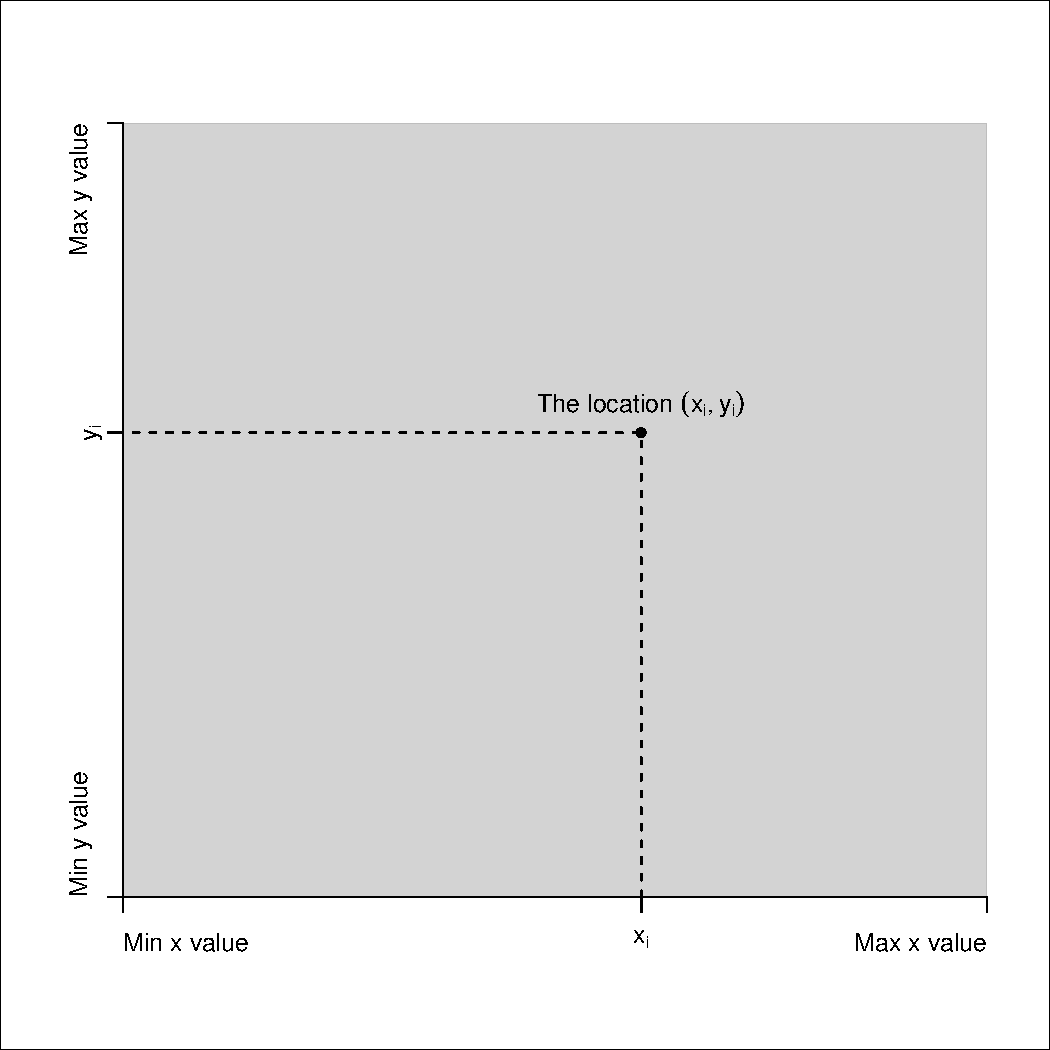
\includegraphics[height=0.95\textheight]{fig3m}
\end{figure}
\end{frame}

\begin{frame}[fragile=singleslide]{Gráficos}{Tipos de linhas
    (\texttt{lty})}
\begin{figure}[htp]
\centering
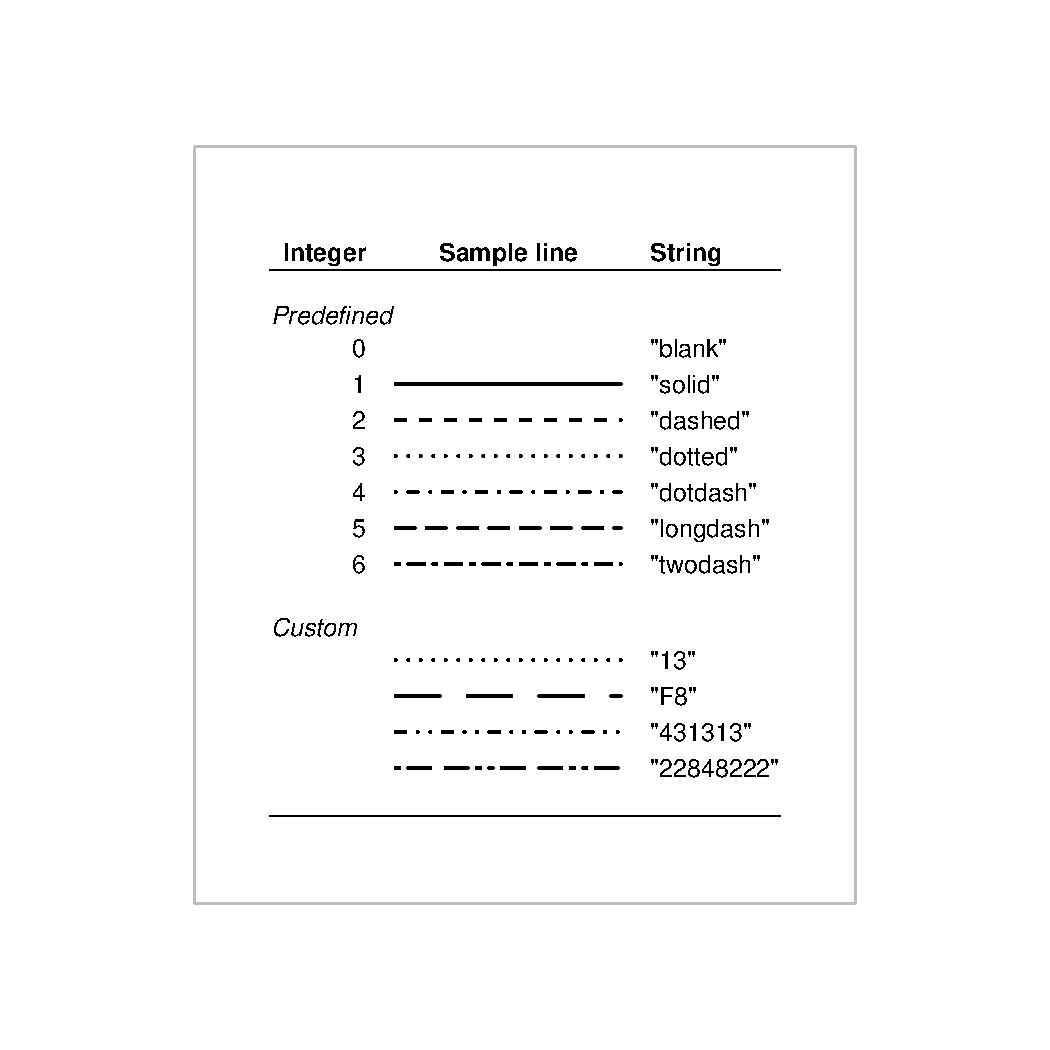
\includegraphics[height=1\textheight]{fig4m}
\end{figure}
\end{frame}

\begin{frame}[fragile=singleslide]{Gráficos}{Tipos de pontos (\texttt{pch})}
\begin{figure}[htp]
\centering
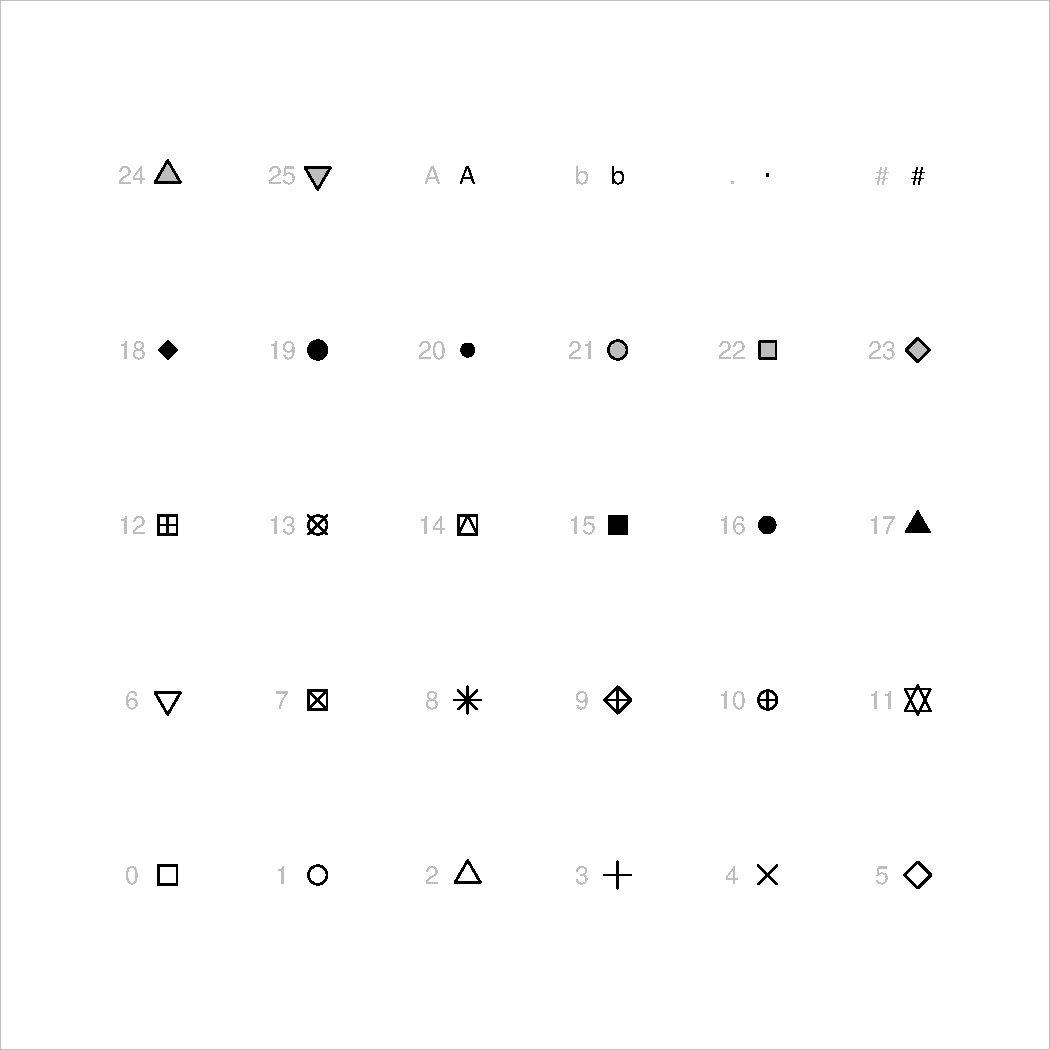
\includegraphics[height=1\textheight]{fig5m}
\end{figure}
\end{frame}

\begin{frame}[fragile=singleslide]{Gráficos}{Tipos de plot (\texttt{type})}
\begin{figure}[htp]
\centering
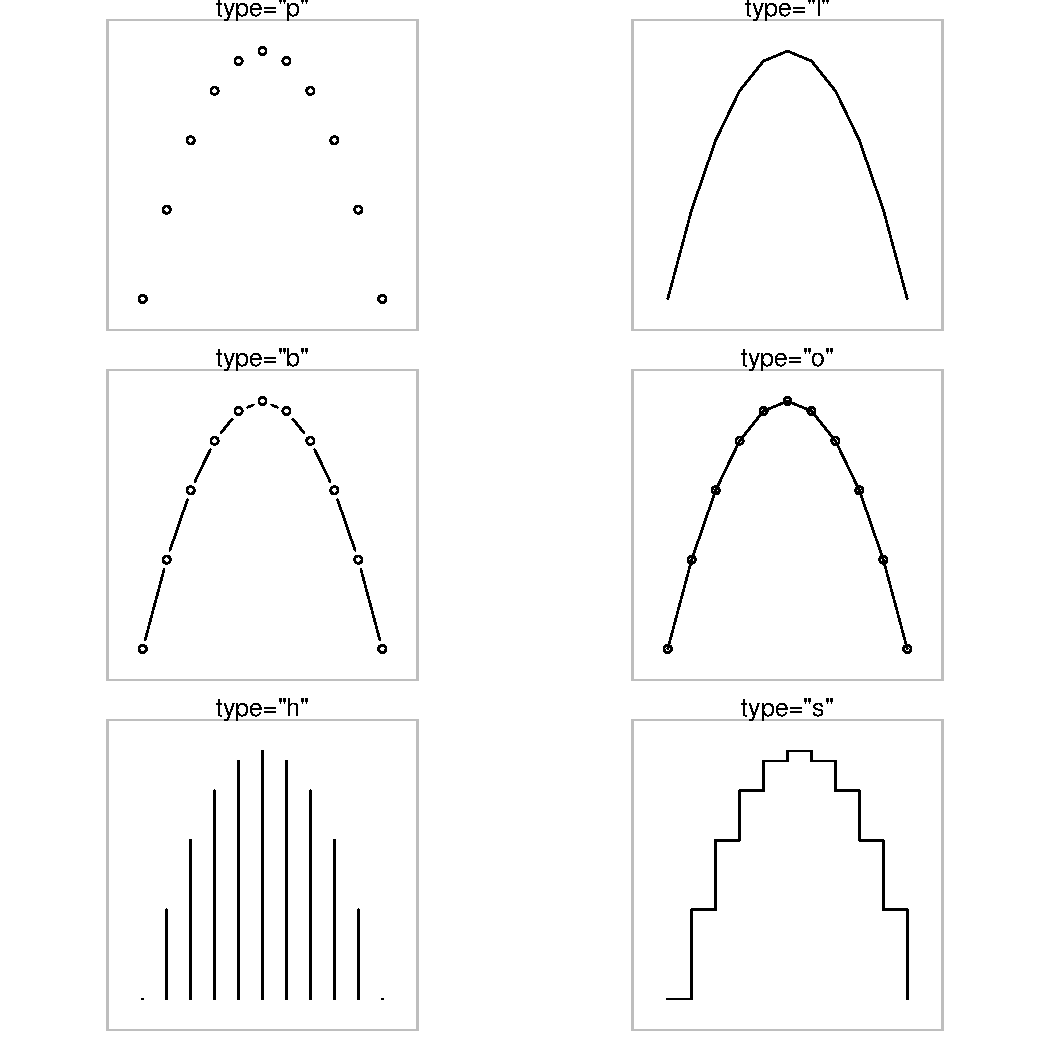
\includegraphics[height=0.95\textheight]{fig6m}
\end{figure}
\end{frame}

\begin{frame}[fragile=singleslide]{Gráficos}{Expressões matemáticas
    (\texttt{expression()})}
\begin{figure}[htp]
\centering
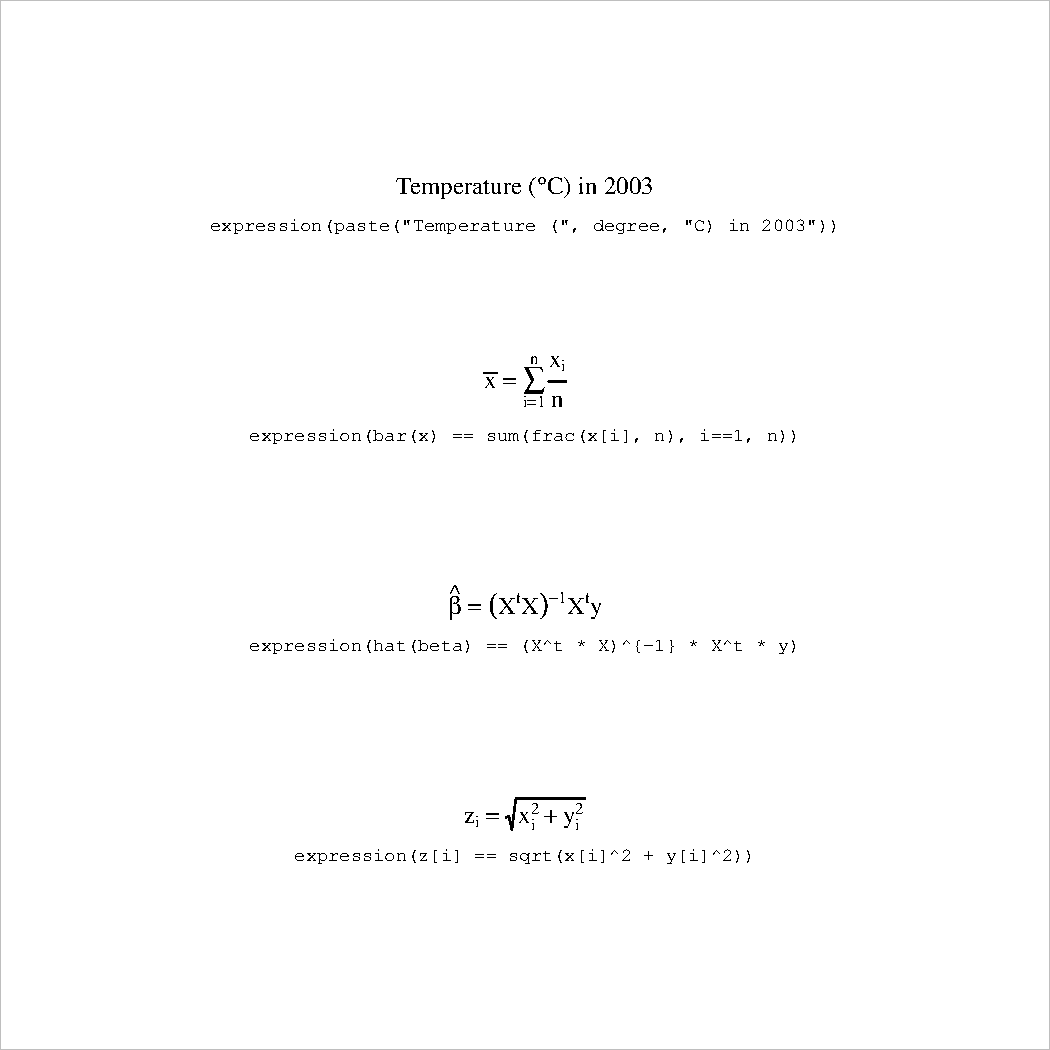
\includegraphics[height=0.95\textheight]{fig7m}
\end{figure}
\end{frame}

\begin{frame}[fragile=singleslide]{A função \texttt{plot()}}
A função \texttt{plot()} é uma \textbf{função genérica}. Os gráficos serão
representados de forma diferente dependendo da \textbf{classe} dos
objetos. A forma geral desta função é:
\begin{knitrout}\small
\definecolor{shadecolor}{rgb}{0.933, 0.914, 0.914}\color{fgcolor}\begin{kframe}
\begin{alltt}
> \hlfunctioncall{plot}(x, y, ...)
\end{alltt}
\end{kframe}
\end{knitrout}

Note que \texttt{y} não precisa ser necessariamente especificado. O
mesmo resultado pode ser obtido em formato de \textbf{fórmula}:
\begin{knitrout}\small
\definecolor{shadecolor}{rgb}{0.933, 0.914, 0.914}\color{fgcolor}\begin{kframe}
\begin{alltt}
> \hlfunctioncall{plot}(y ~ x, data, ...)
\end{alltt}
\end{kframe}
\end{knitrout}

Onde lê-se ``\texttt{y} descrito utilizando-se \texttt{x}'', ou
``\texttt{y} em função de \texttt{x}''
\end{frame}

\begin{frame}[fragile=singleslide]{A função \texttt{plot()}}
\begin{knitrout}\small
\definecolor{shadecolor}{rgb}{0.933, 0.914, 0.914}\color{fgcolor}\begin{kframe}
\begin{alltt}
> \hlfunctioncall{plot}(dados)
\end{alltt}
\end{kframe}

{\centering 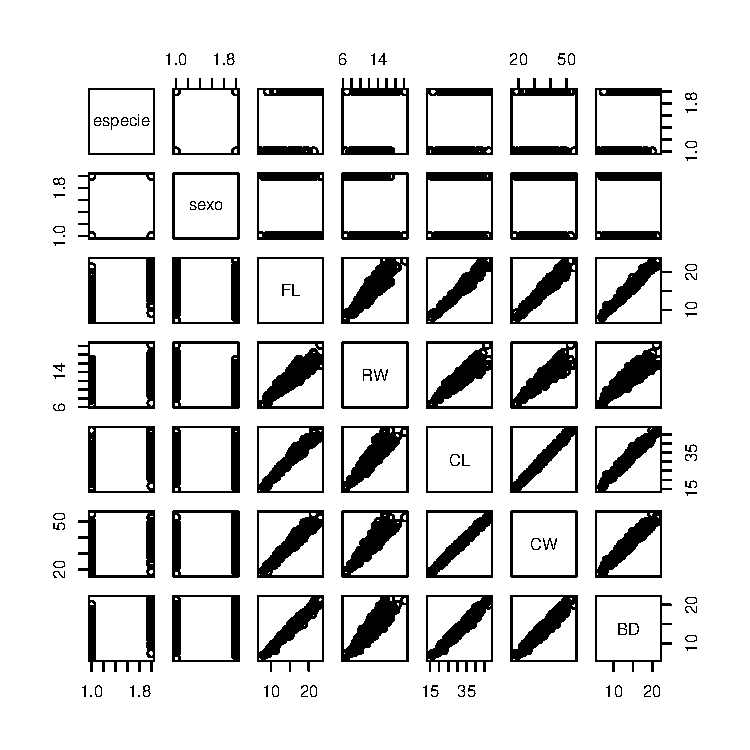
\includegraphics[width=.7\textwidth]{figure/unnamed-chunk-25} 

}


\end{knitrout}

\end{frame}

\begin{frame}[fragile=singleslide]{A função \texttt{plot()}}
\begin{knitrout}\small
\definecolor{shadecolor}{rgb}{0.933, 0.914, 0.914}\color{fgcolor}\begin{kframe}
\begin{alltt}
> \hlfunctioncall{plot}(dados$CL)     \hlcomment{# uma variável}
\end{alltt}
\end{kframe}

{\centering 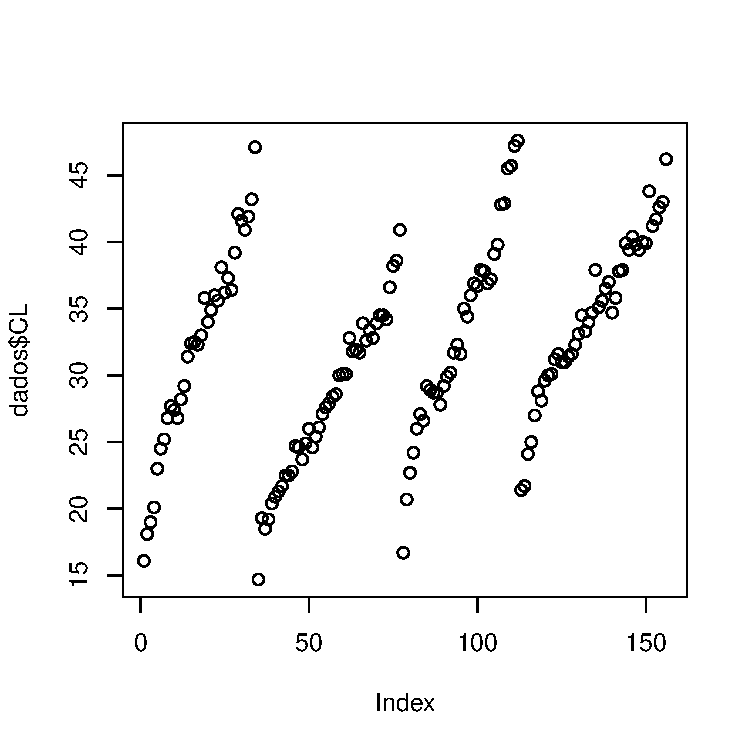
\includegraphics[width=.7\textwidth]{figure/unnamed-chunk-26} 

}


\end{knitrout}

\end{frame}

\begin{frame}[fragile=singleslide]{A função \texttt{plot()}}
\begin{knitrout}\small
\definecolor{shadecolor}{rgb}{0.933, 0.914, 0.914}\color{fgcolor}\begin{kframe}
\begin{alltt}
> \hlfunctioncall{plot}(dados$CL, dados$CW)    \hlcomment{# duas variáveis, ou:}
> \hlfunctioncall{plot}(CW ~ CL, data = dados) \hlcomment{# mesmo resultado}
\end{alltt}
\end{kframe}

{\centering 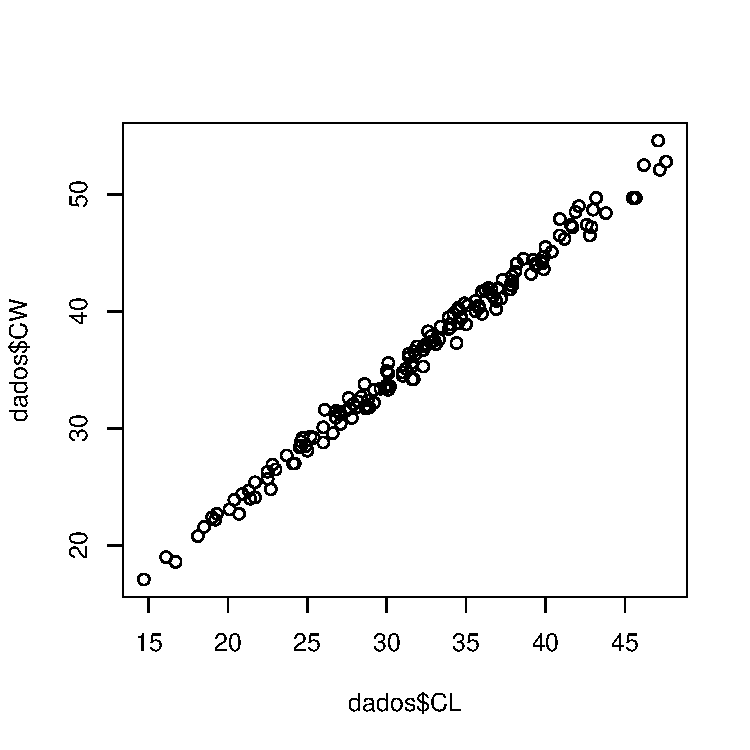
\includegraphics[width=.49\textwidth]{figure/unnamed-chunk-271} 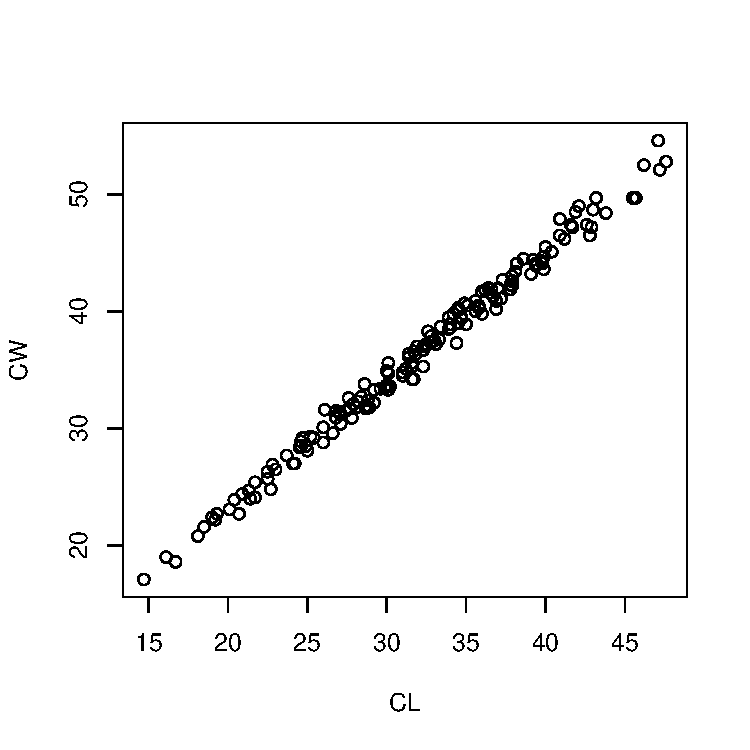
\includegraphics[width=.49\textwidth]{figure/unnamed-chunk-272} 

}


\end{knitrout}

\end{frame}

\begin{frame}[fragile=singleslide]{A função \texttt{plot()}}
\begin{knitrout}\small
\definecolor{shadecolor}{rgb}{0.933, 0.914, 0.914}\color{fgcolor}\begin{kframe}
\begin{alltt}
> \hlfunctioncall{plot}(dados$especie, dados$CL)  \hlcomment{# fator, numérico}
\end{alltt}
\end{kframe}

{\centering 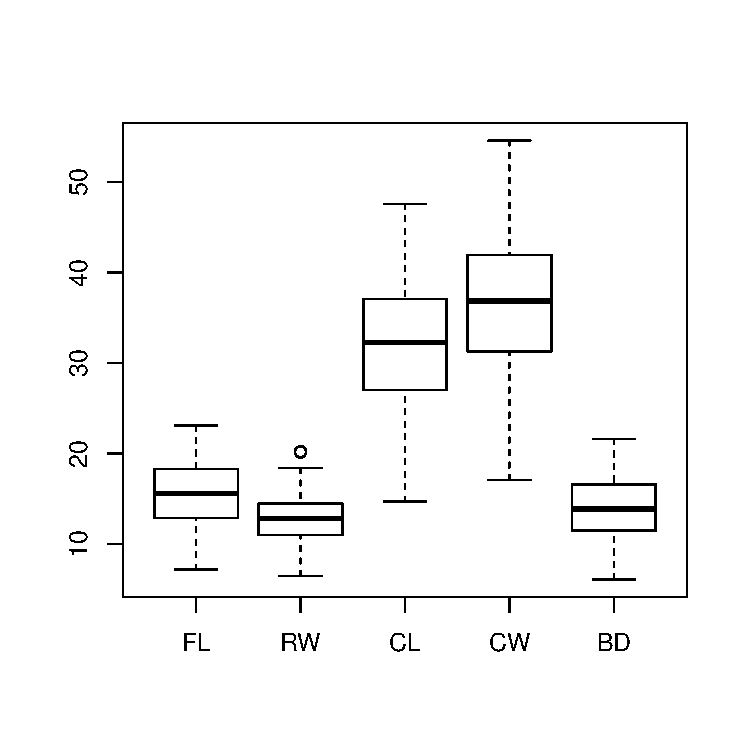
\includegraphics[width=.7\textwidth]{figure/unnamed-chunk-28} 

}


\end{knitrout}

\end{frame}

\begin{frame}[fragile=singleslide]{A função \texttt{boxplot()}}
Os \textbf{boxplots} são úteis para revelar o centro, a dispersão e a
distribuição dos dados, além de \textbf{outliers}. São construídos da
seguinte forma:
\begin{itemize}
\item A linha central mais escura representa a mediana. Os extremos da
  caixa são o $1^{o}$ ($q1$) e o $3^{o}$ ($q3$) quartis.
\item As linhas que se extendem das caixas são definidas como:
\begin{displaymath}
q1-1,5\cdot IQR\ \qquad \mathrm{e}\ \qquad q3+1,5\cdot IQR
\end{displaymath}
onde $IQR$ é o intervalo inter-quartil. As linhas vão até os valores
máximo e mínimo que ainda se encontram dentro deste intervalo.
\end{itemize}
\end{frame}

% \begin{frame}[fragile=singleslide]{(Adicionando novas colunas)}
% Calcule a CPUE das três espécies:
% \begin{verbatim}
% dados$u.lage <- (dados$lage*1000)/dados$eff
% dados$u.branca <- (dados$branca*1000)/dados$eff
% dados$u.bandolim <- (dados$bandolim*1000)/dados$eff
% \end{verbatim}
% \end{frame}

\begin{frame}[fragile=singleslide]{A função \texttt{boxplot()}}
\begin{knitrout}\small
\definecolor{shadecolor}{rgb}{0.933, 0.914, 0.914}\color{fgcolor}\begin{kframe}
\begin{alltt}
> \hlfunctioncall{boxplot}(dados[, 3:7])
\end{alltt}
\end{kframe}

{\centering 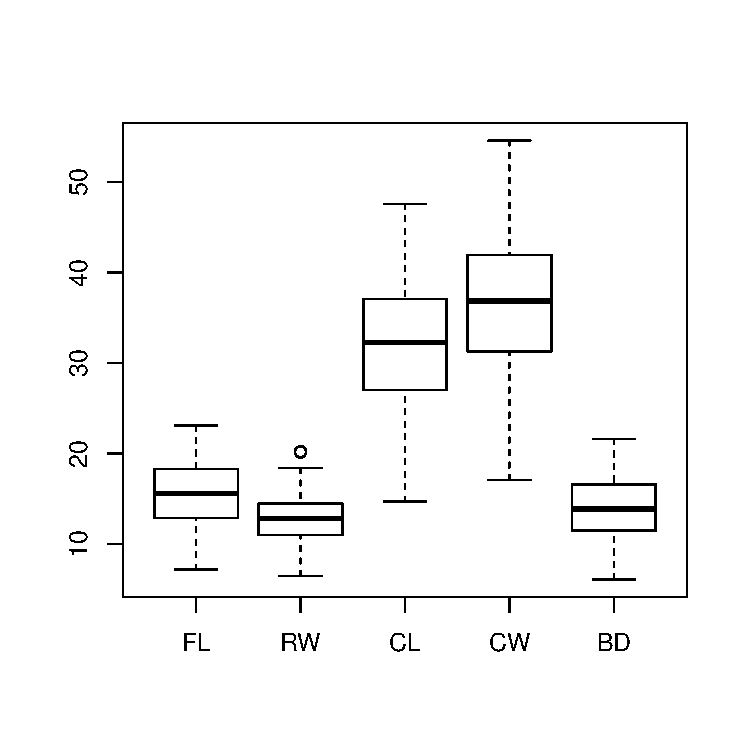
\includegraphics[width=.7\textwidth]{figure/unnamed-chunk-29} 

}


\end{knitrout}

\end{frame}

\begin{frame}[fragile=singleslide]{A função \texttt{boxplot()}}
\begin{knitrout}\small
\definecolor{shadecolor}{rgb}{0.933, 0.914, 0.914}\color{fgcolor}\begin{kframe}
\begin{alltt}
> \hlfunctioncall{boxplot}(CL ~ especie, data = dados)        \hlcomment{# um fator}
> \hlfunctioncall{boxplot}(CL ~ especie + sexo, data = dados) \hlcomment{# dois fatores}
\end{alltt}
\end{kframe}

{\centering 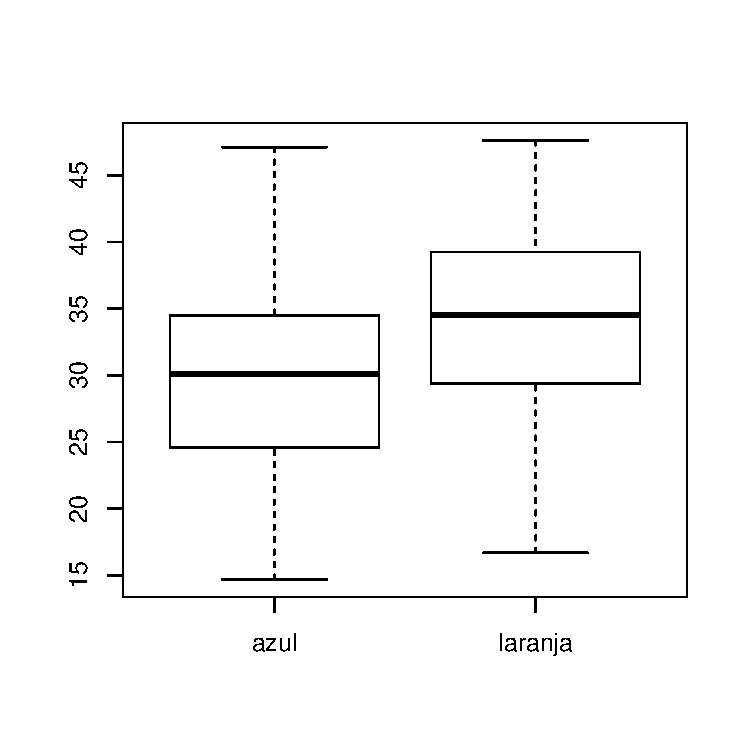
\includegraphics[width=.49\textwidth]{figure/unnamed-chunk-301} 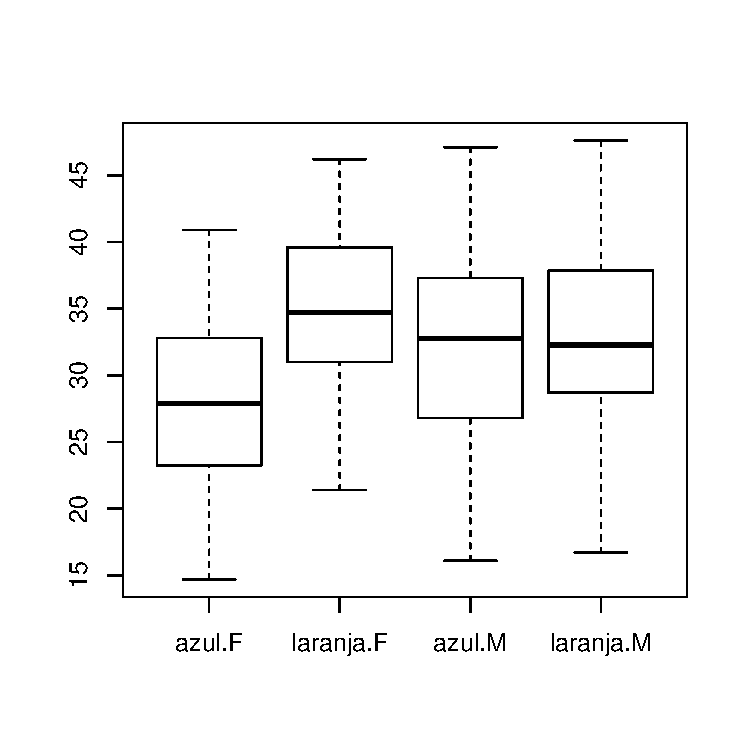
\includegraphics[width=.49\textwidth]{figure/unnamed-chunk-302} 

}


\end{knitrout}

\end{frame}

\begin{frame}[fragile=singleslide]{A função \texttt{hist()}}
Na função \texttt{hist()}, dois argumentos controlam a configuração das
classes:
\begin{center}
\begin{table}[h!]
\begin{tabular}{c|c}
\hline
Argumentos & resultado \\
\hline
\texttt{include.lowest = T, right = T} & \texttt{[a,b], ..., (c,d]} \\
\texttt{include.lowest = F, right = T} & \texttt{(a,b], ..., (c,d]} \\
\texttt{include.lowest = F, right = F} & \texttt{[a,b), ..., [c,d)} \\
\texttt{include.lowest = T, right = F} & \texttt{[a,b), ..., [c,d]} \\
\hline
\end{tabular}
\end{table}
\end{center}
O argumento \texttt{breaks} também pode ser utilizado para especificar
as ``quebras'' das classes.
\end{frame}

\begin{frame}[fragile=singleslide]{A função \texttt{hist()}}
\begin{knitrout}\small
\definecolor{shadecolor}{rgb}{0.933, 0.914, 0.914}\color{fgcolor}\begin{kframe}
\begin{alltt}
> \hlfunctioncall{hist}(dados$CL)
\end{alltt}
\end{kframe}

{\centering 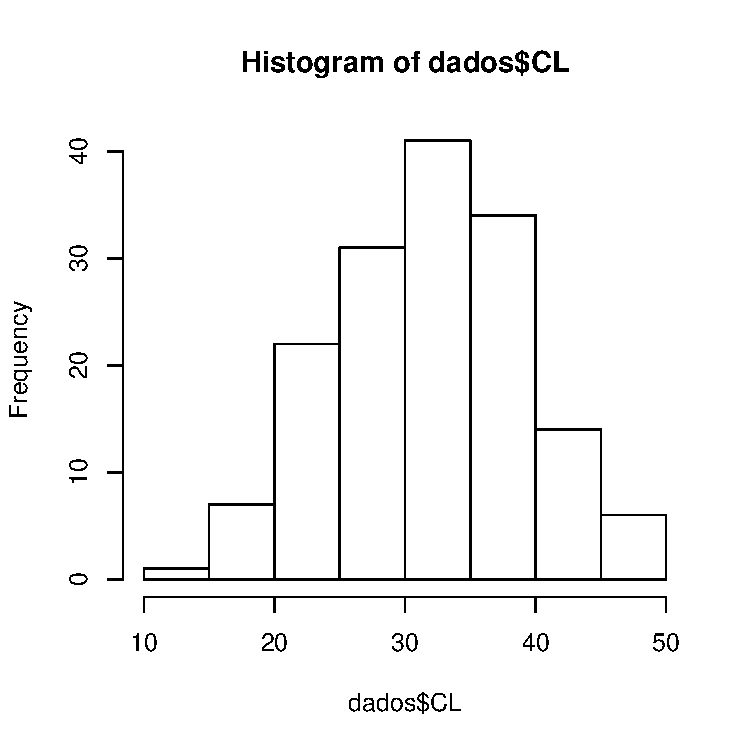
\includegraphics[width=.7\textwidth]{figure/unnamed-chunk-31} 

}


\end{knitrout}

\end{frame}

\begin{frame}[fragile=singleslide]{A função \texttt{hist()}}
\begin{knitrout}\small
\definecolor{shadecolor}{rgb}{0.933, 0.914, 0.914}\color{fgcolor}\begin{kframe}
\begin{alltt}
> \hlfunctioncall{hist}(dados$CL, breaks = \hlfunctioncall{seq}(10, 50, 1)) \hlcomment{# ou}
> \hlfunctioncall{hist}(dados$CL, nclass = 40)             \hlcomment{# aproximado}
\end{alltt}
\end{kframe}

{\centering 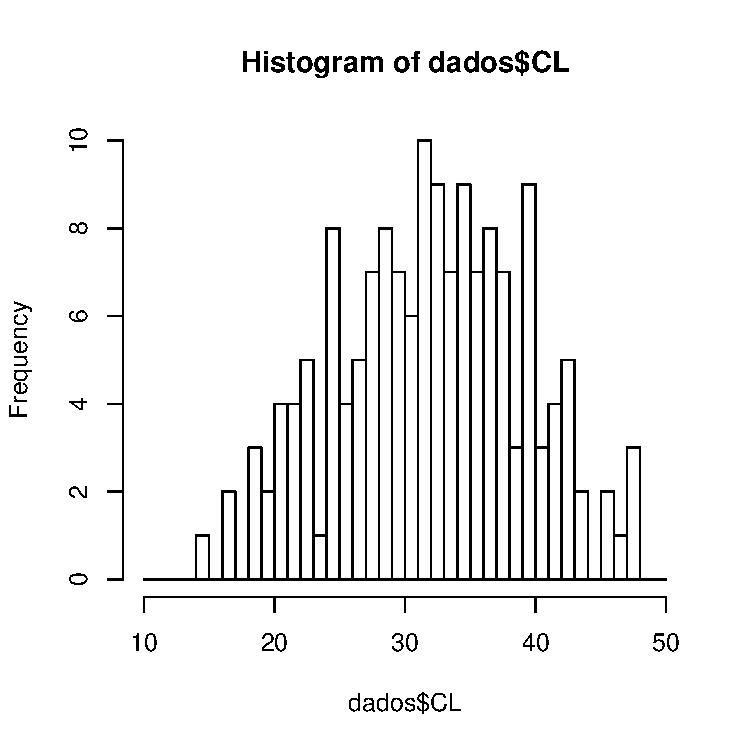
\includegraphics[width=.49\textwidth]{figure/unnamed-chunk-321} 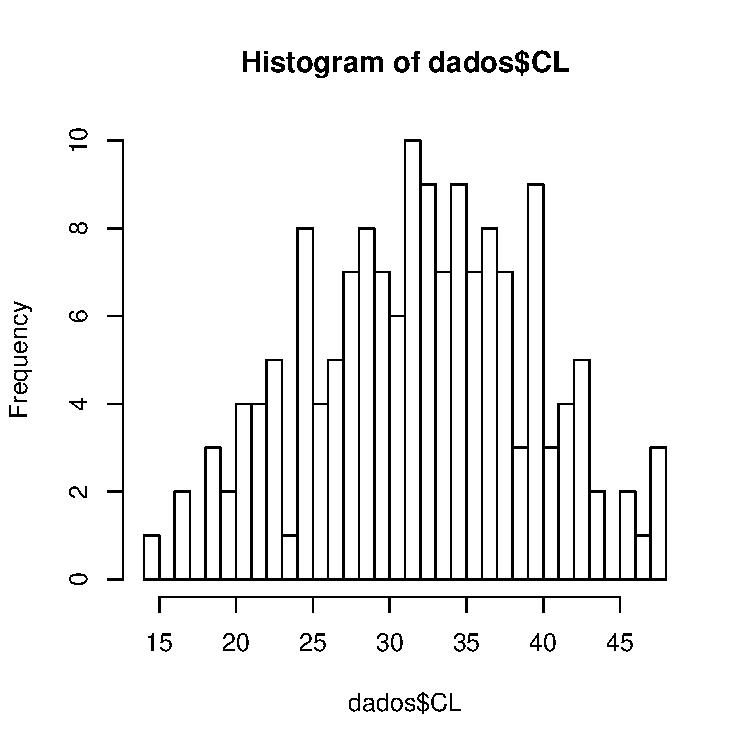
\includegraphics[width=.49\textwidth]{figure/unnamed-chunk-322} 

}


\end{knitrout}

\end{frame}

\begin{frame}[fragile=singleslide]{A função \texttt{hist()}}
A função \texttt{hist()}, além de produzir histogramas também retorna
uma lista com as uma série de informações:
\begin{knitrout}\small
\definecolor{shadecolor}{rgb}{0.933, 0.914, 0.914}\color{fgcolor}\begin{kframe}
\begin{alltt}
> h <- \hlfunctioncall{hist}(dados$CL)
> h
\end{alltt}
\begin{verbatim}
$breaks
[1] 10 15 20 25 30 35 40 45 50

$counts
[1]  1  7 22 31 41 34 14  6

$intensities
[1] 0.0012821 0.0089744 0.0282051 0.0397436 0.0525641 0.0435897
[7] 0.0179487 0.0076923

$density
[1] 0.0012821 0.0089744 0.0282051 0.0397436 0.0525641 0.0435897
[7] 0.0179487 0.0076923

$mids
[1] 12.5 17.5 22.5 27.5 32.5 37.5 42.5 47.5

$xname
[1] "dados$CL"

$equidist
[1] TRUE

attr(,"class")
[1] "histogram"
\end{verbatim}
\end{kframe}
\end{knitrout}

\end{frame}

\begin{frame}[fragile=singleslide]{A função \texttt{hist()}}
\begin{knitrout}\small
\definecolor{shadecolor}{rgb}{0.933, 0.914, 0.914}\color{fgcolor}\begin{kframe}
\begin{alltt}
> \hlfunctioncall{hist}(dados$CL)           \hlcomment{# contagem}
> \hlfunctioncall{hist}(dados$CL, freq = F) \hlcomment{# densidade}
\end{alltt}
\end{kframe}

{\centering 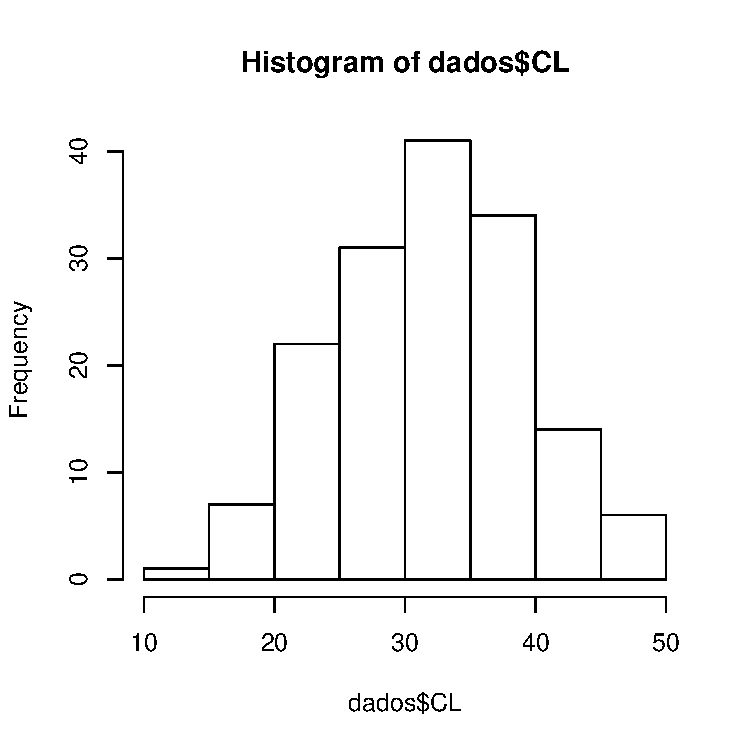
\includegraphics[width=.49\textwidth]{figure/unnamed-chunk-341} 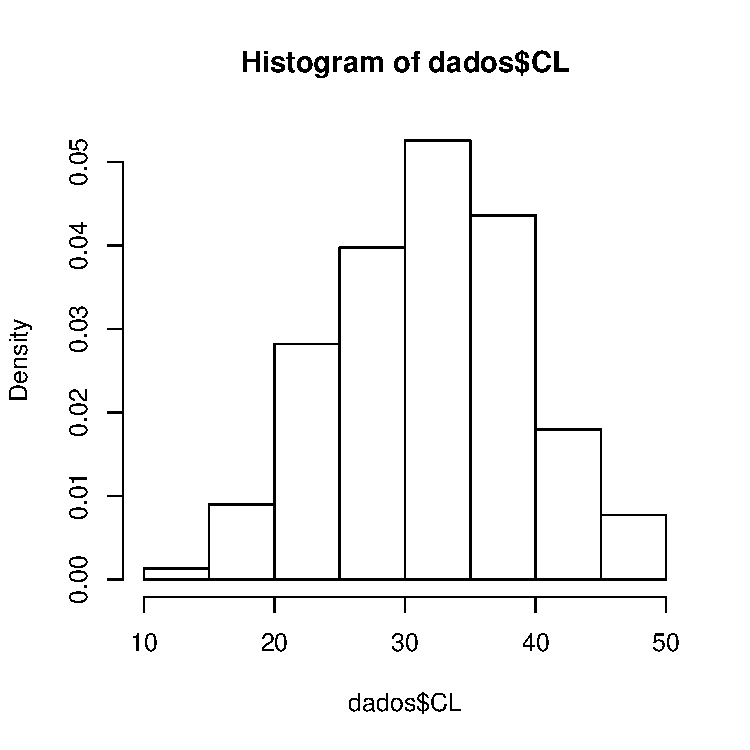
\includegraphics[width=.49\textwidth]{figure/unnamed-chunk-342} 

}


\end{knitrout}

\end{frame}

\begin{frame}[fragile=singleslide]{A função \texttt{barplot()}}
A função \texttt{barplot()} gera gráficos de barra a partir de uma
tabela
\begin{knitrout}\small
\definecolor{shadecolor}{rgb}{0.933, 0.914, 0.914}\color{fgcolor}\begin{kframe}
\begin{alltt}
> \hlfunctioncall{table}(dados$especie)
\end{alltt}
\begin{verbatim}

   azul laranja 
     77      79 
\end{verbatim}
\begin{alltt}
> \hlfunctioncall{barplot}(\hlfunctioncall{table}(dados$especie))
\end{alltt}
\end{kframe}

{\centering 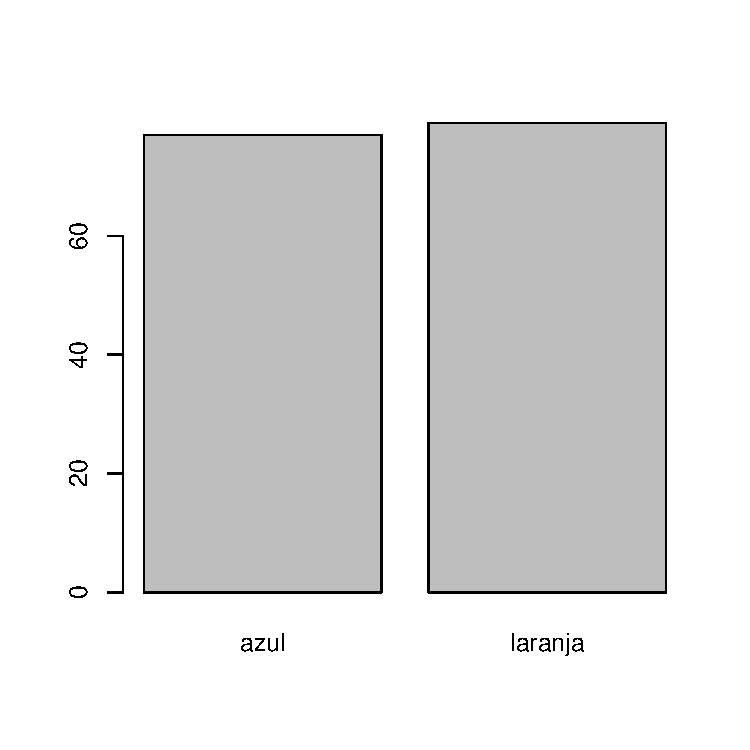
\includegraphics[width=.45\textwidth]{figure/unnamed-chunk-35} 

}


\end{knitrout}

\end{frame}

\begin{frame}[fragile=singleslide]{A função \texttt{barplot()}}
\begin{knitrout}\small
\definecolor{shadecolor}{rgb}{0.933, 0.914, 0.914}\color{fgcolor}\begin{kframe}
\begin{alltt}
> \hlfunctioncall{table}(dados$especie, dados$sexo)
\end{alltt}
\begin{verbatim}
         
           F  M
  azul    43 34
  laranja 44 35
\end{verbatim}
\begin{alltt}
> \hlfunctioncall{barplot}(\hlfunctioncall{table}(dados$especie, dados$sexo))
> \hlfunctioncall{barplot}(\hlfunctioncall{table}(dados$especie, dados$sexo), beside = T)
\end{alltt}
\end{kframe}

{\centering 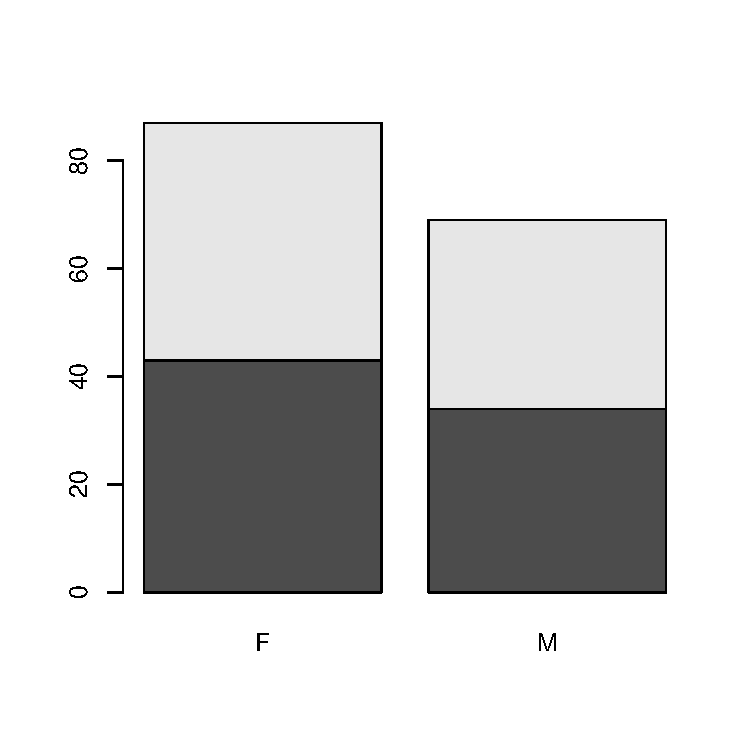
\includegraphics[width=.4\textwidth]{figure/unnamed-chunk-361} 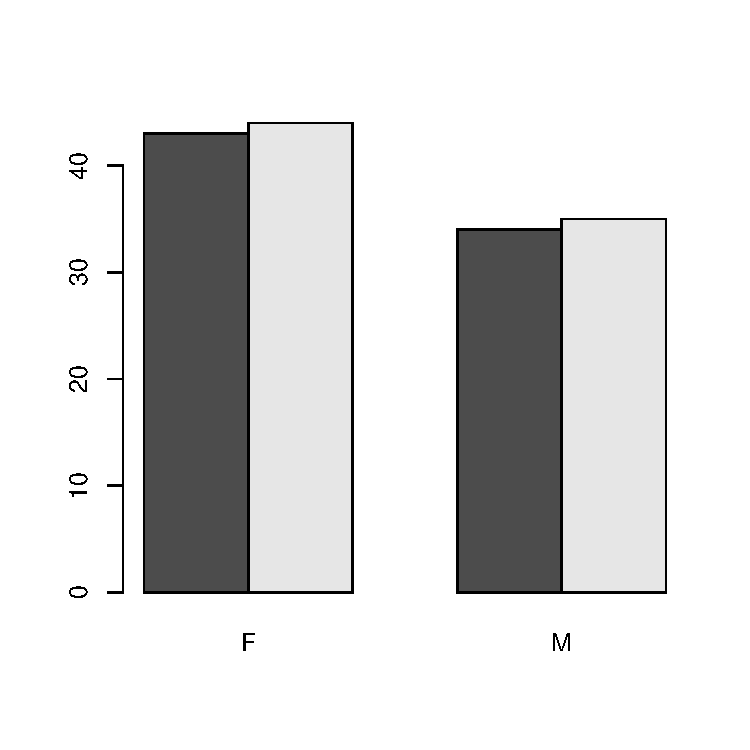
\includegraphics[width=.4\textwidth]{figure/unnamed-chunk-362} 

}


\end{knitrout}

\end{frame}

                                % ADICIONAR: Controle sobre os graficos

\subsection{Argumentos gráficos}

\begin{frame}[fragile=singleslide]{Argumentos gráficos}
  Os principais argumentos que servem uma grande quantidade de funções
  gráficas são
  \begin{itemize}
  \item \texttt{xlab}, \texttt{ylab}: (\verb|"caracter"|) alteram o nome
    dos eixos (\texttt{x} e \texttt{y} \texttt{lab}el)
  \item \texttt{xlim}, \texttt{ylim}: (\verb|c(min, max)|) alteram os
    limites dos eixos (\texttt{x} e \texttt{y} \texttt{lim}its)
  \item \texttt{main}: (\verb|"caracter"|) altera o título do gráfico
  \end{itemize}
\end{frame}

\begin{frame}[fragile=singleslide]{Argumentos gráficos}
\begin{knitrout}\small
\definecolor{shadecolor}{rgb}{0.933, 0.914, 0.914}\color{fgcolor}\begin{kframe}
\begin{alltt}
> \hlfunctioncall{plot}(dados$CL, dados$CW,
       xlab = \hlstring{"Comprimento da \hlfunctioncall{carapaça} (cm)"},
       ylab = \hlstring{"Largura da \hlfunctioncall{carapaça} (cm)"},
       main = \hlstring{"Relação entre CL e CW"})
\end{alltt}
\end{kframe}

{\centering 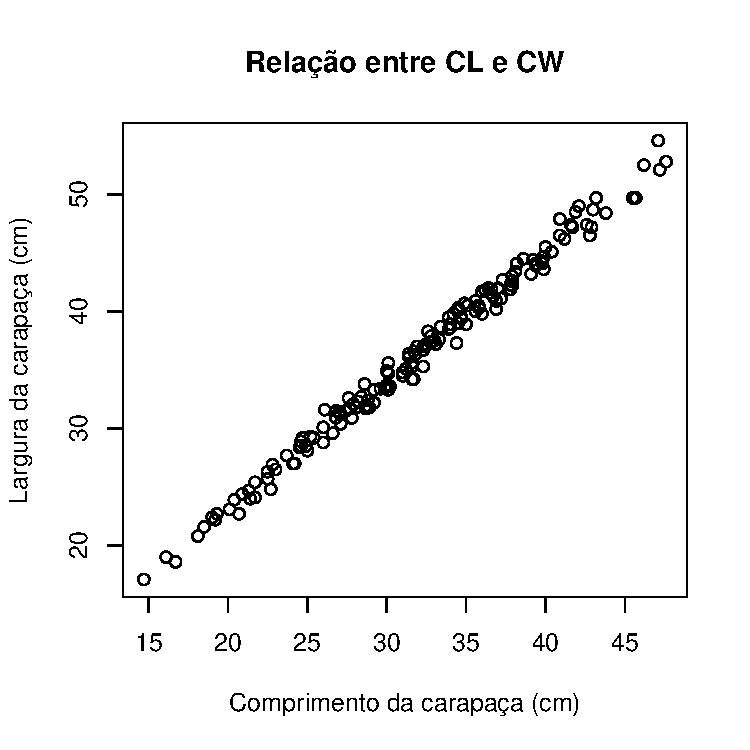
\includegraphics[width=.55\textwidth]{figure/unnamed-chunk-37} 

}


\end{knitrout}

\end{frame}

\begin{frame}[fragile=singleslide]{Argumentos gráficos}
\begin{knitrout}\small
\definecolor{shadecolor}{rgb}{0.933, 0.914, 0.914}\color{fgcolor}\begin{kframe}
\begin{alltt}
> \hlfunctioncall{hist}(dados$CL, main = \hlstring{""}, xlim = \hlfunctioncall{c}(0, 60),
       xlab = \hlstring{"Comprimento da \hlfunctioncall{carapaça} (cm)"},
       ylab = \hlstring{"Frequência"})
\end{alltt}
\end{kframe}

{\centering 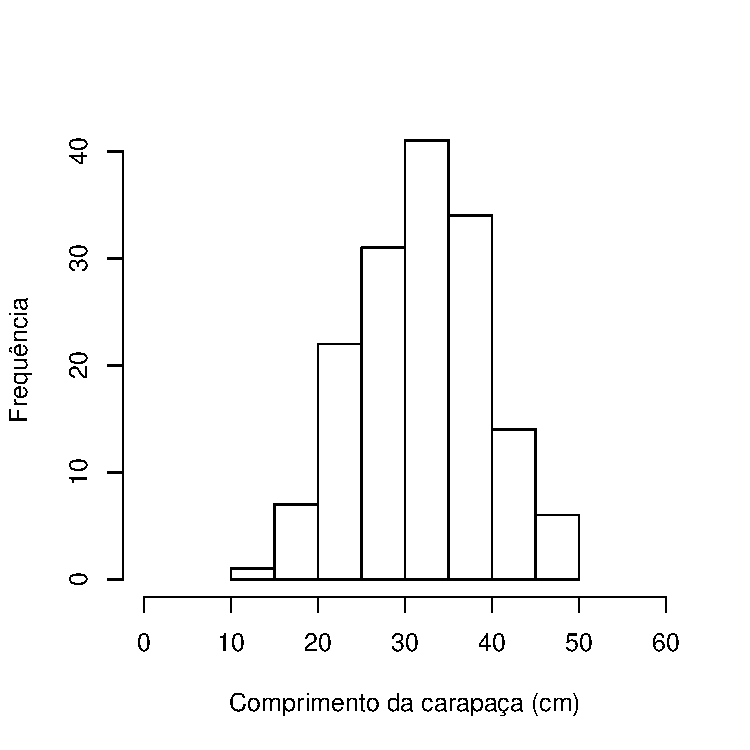
\includegraphics[width=.55\textwidth]{figure/unnamed-chunk-38} 

}


\end{knitrout}

\end{frame}

\subsection{Outros pacotes gráficos}

\begin{frame}[fragile=singleslide]{Ouros pacotes gráficos}
Além do pacote de gráficos padrão do R, \textbf{graphics}, existem
outros que incorporam opções mais avançadas
\begin{itemize}
\item \textbf{lattice} (mais antigo)
\item \textbf{ggplot2} (mais recente)
\end{itemize}
\end{frame}

% \section{Programação}

% \begin{frame}{Programação}
% \setbeamercovered{dynamic} % para shades depois do pause
%   \begin{itemize}
%   \item Por quê programar?
%     \begin{itemize}
%     \item Evitar repetições desnecessárias de análises ou cálculos que
%       são repetidos com frequência.
%     \item Fica documentado as etapas que você realizou para chegar a um
%       resultado.
%     \item Fácil recuperação e modificação de programas.
%     \end{itemize}\pause
%   \item Como programar?
%     \begin{itemize}
%     \item Criando programas! (Scripts, rotinas, \textbf{algoritmos}).
%     \item Crie uma sequência lógica de comandos que devem ser executados
%       em ordem.
%     \item Utilize as ferramentas básicas da programação:
%       \textbf{estruturas de repetição} (\texttt{for()}) e
%       \textbf{estruturas de seleção} (\texttt{if()}).
%     \end{itemize}
%   \end{itemize}
% \end{frame}

% \begin{frame}[fragile=singleslide]{Estrutura de repetição
%     \texttt{for()}}
%   \begin{itemize}
%   \item Serve para repetir um ou mais comandos diversas vezes.
%   \item Exemplo: cálculo de notas de uma disciplina.
%   \end{itemize}
% \begin{verbatim}
% # importa os dados
% notas <- read.table("notas.csv", header = TRUE,
%                     sep=";", dec=",")
% # cria uma nova coluna para armazenar os resultados
% notas$media <- 0
% # estrutura de repetição
% for(i in 1:30){
%     notas$media[i] <- sum(notas[i, c("prova1",
%                                      "prova2",
%                                      "prova3")])/3
% }
% \end{verbatim}
% \end{frame}

% \begin{frame}[fragile=singleslide]{Estrutura de repetição
%     \texttt{for()}}
%   \begin{itemize}
%   \item Inserindo pesos para as provas: prova 1 = 4, prova 2 = 3, prova
%     3 = 3.
%   \end{itemize}
% \begin{verbatim}
% # estrutura de repetição
% for(i in 1:30){
%     pesos <- notas[i, c("prova1", "prova2", "prova3")]
%     * c(4,3,3)
%     notas$media[i] <- sum(pesos)/10
% }
% \end{verbatim}
% \end{frame}

% \begin{frame}[fragile=singleslide]{Estrutura de seleção \texttt{if()}}
%   \begin{itemize}
%   \item Adicionando a condição do aluno de acordo com a nota.
%   \end{itemize}
% \begin{verbatim}
% # nova coluna para armazenar os resultados
% notas$situacao <- NA
% # estrutura de repetição
% for(i in 1:30){
%     pesos <- notas[i, c("prova1", "prova2", "prova3")] *
%         c(4,3,3)
%     notas$media[i] <- sum(pesos)/10
%     # estrutura de seleção
%     if(notas$media[i] >= 7){
%         notas$situacao[i] <- "aprovado"
%     } else{
%         notas$situacao[i] <- "reprovado"
%     }
% }
% \end{verbatim}
% \end{frame}

%% \begin{frame}[fragile=singleslide]{O modo de R --- Vetorização}
%%   \begin{itemize}
%%   \item Através do processo de vetorização do R, o mesmo algoritmo pode
%%     ser simplificado em duas etapas.
%%   \end{itemize}
%% \begin{verbatim}

%% \end{verbatim}
%% \end{frame}


\end{document}
